\section{\Sys Design}
\label{sec:methodology}

\Sys, depicted in Figure \ref{arch}, comprises four key modules: a provenance graph constructor, a Semantic Vectors Harmonization, Federated Learning Module, and Anomaly Detection. The main server is responsible for initiating the global model weights, which are then transmitted to the client machines. The clients use these weights as their starting point and conduct model training on their respective local datasets. Subsequently, the clients send their updated weights back to the main server for federated averaging.

In addition to the primary task, each client machine also trains a word2vec model to feature semantic attributes in audit logs. It's noteworthy that the word2vec models on different clients may yield distinct embeddings for the same tokens. To address this potential non-iid data problem, \Sys employs the utility server to harmonize these models.

\subsection{Provenance Graph Constructor}
Our approach starts by converting system logs into provenance graphs through a three-step process. Initially, the system, \Sys, processes system logs like Windows Event Logs or Linux Audit Logs, which are composed of host event details including process activities, file interactions, and network engagements. \Sys works with batches of audit logs, utilizing a sliding window technique to create the provenance graph. This graph consists of two kinds of nodes: process nodes and object nodes. The object nodes represent various system entities such as files, network streams, modules, and other system components. The connections between these nodes are marked with labels indicating the event type, elucidating the cause-and-effect relationship among the connected nodes and the event's timestamp. Additionally, these nodes are equipped with attributes like process identifiers, command lines, file paths, IP addresses, port details, and module paths, offering additional insights and specifics.

\subsection{Semantic Vectors Harmonization}
Our system employs the word2vec model to encode various semantic attributes into a vector space, which is pivotal in distinguishing normal system entities from anomalies. Traditional approaches utilize a centralized word2vec model for this encoding. However, in a federated learning context, complexities arise as each individual client must train its word2vec model for attribute encoding. Consequently, different clients might encode the same attributes into diverse vectors, leading to a non-Independent and Identically Distributed (Non-IID) problem. This variation hampers the convergence of the Graph Neural Network (GNN) model in federated learning scenarios. 

To address this issue, we have developed a technique leveraging a utility server to synchronize disparate models across clients. This approach achieves uniformity in encoding the same attributes while preserving privacy, as clients are not required to share their attributes. The process initiates with the main server distributing an encryption and decryption key to each client. Clients then encrypt their word2vec model tokens, concealing their meanings. Subsequently, these encrypted models are sent to the utility server, which remains unaware of the encryption key used. The utility server then averages the vectors for the corresponding encrypted tokens, creating a unified and harmonized word2vec model. Finally, this model is returned to the clients, who utilize the decryption key to revert their encrypted tokens to their original attributes.

\subsection{Federated Learning Module}
Each client machine independently trains a \gnn model on a provenance graph built from its local log data, thereby preserving privacy. These individually trained models are then sent to the main server. Upon receiving them, the main server applies a federated averaging algorithm to integrate these models into a single, centralized model. This unified model is subsequently distributed back to each client. This cycle of training and unification is repeated over several rounds until the model reaches convergence. Finally, clients employ the fully trained model to perform anomaly detection.

\subsection{Anomaly Detection}
\Sys utilizes an advanced approach to pinpoint irregular nodes by assessing the disparity between their expected and observed types. This method is rooted in a thorough examination of the surrounding structures and intrinsic qualities of nodes, aiming to establish a baseline of normal patterns for various node classifications. It is observed that entities with malicious intent often manifest neighborhood configurations and characteristics that are inconsistent with these established norms. During operational phases, encountering such anomalies that stand apart from the pre-learned node distribution patterns leads to their erroneous classification. The presence of nodes incorrectly categorized in the output serves as an indicator of potential security concerns. We have introduced a regulatory mechanism in the form of a threshold parameter, $T$, to oversee the frequency of alerts. This parameter effectively caps the classification likelihood for a given prediction. A higher parameter value correlates with stronger conviction in the prediction, signaling a greater chance of uncovering anomalies.


\begin{figure}[t!]
    \centering
    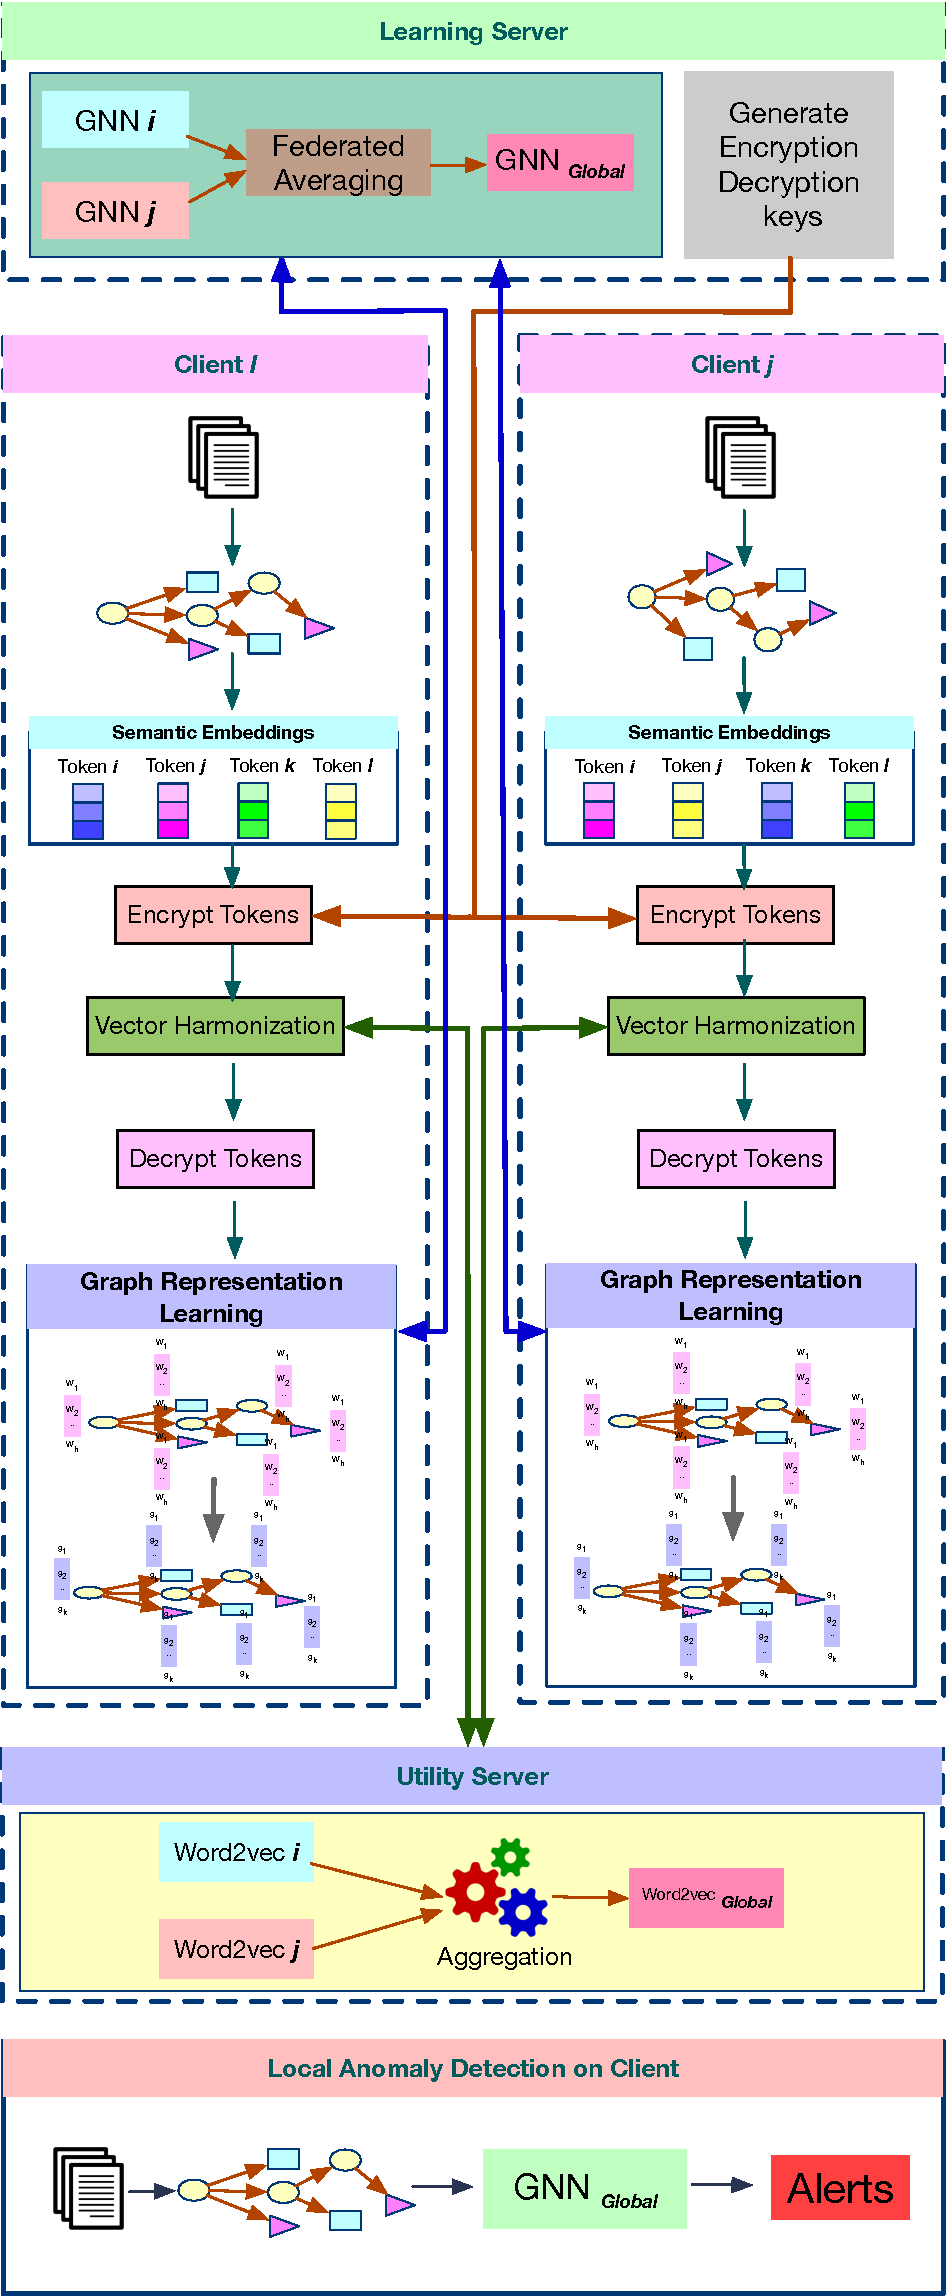
\includegraphics[width=0.45\textwidth]{fig/arch.pdf}
    \caption{High Level Architecture of \Sys}
    \vspace{-3ex}
    \label{arch}
  \end{figure}
